% !TEX root = ../Thesis.tex
\newcommand{\rphi}{\ensuremath{R\textrm{-}\phi}}
\newcommand{\T}{\ensuremath{\mathbf{T}}}
\newcommand{\Tms}{\ensuremath{\T_{\textrm{MS}}}}
\newcommand{\Tid}{\ensuremath{\T_{\textrm{ID}}}}
\newcommand{\C}{\ensuremath{\mathbf{C}}}
\newcommand{\Cms}{\ensuremath{\C_{\textrm{MS}}}}
\newcommand{\Cid}{\ensuremath{\C_{\textrm{ID}}}}
\newcommand{\kt}{\ensuremath{k_{\textrm{T}}}}
\newcommand{\kti}{\ensuremath{k_{\textrm{T},i}}}
\newcommand{\ktj}{\ensuremath{k_{\textrm{T},j}}}
\newcommand{\dij}{\ensuremath{\Delta_{ij}}}

\chapter{The LHC and the ATLAS Detector} \label{ch:Detector}

The Large Hadron Collider (LHC)~\cite{LHC} is a proton-proton ring collider located at the European Centre for Nuclear Research (CERN). The main LHC ring is housed in the tunnel which previously contained the Large Electron-Positron collider. The LHC ring is \SI{27}{\kilo\meter} in circumference and located as deep as \SI{175}{\meter} underground. The LHC services seven different experiments located around the beam-pipe (Figure~\ref{fig:DetectorLHCLayout}). The four main experiments are: A toroidal LHC apparatus (ATLAS, the experiment used for this thesis), the compact muon solenoid (CMS), a large ion collider (ALICE) experiment and the LHC beauty (LHCb) experiment. 

ATLAS and CMS are general purpose detectors designed to support a varied physics programme, from SM physics like top quark measurements to BSM searches such as supersymmetry. ALICE and LHCb are more specialized experiments which focus on heavy ions and $B$-physics, respectively.

\begin{figure}[htbp]
  \centering
    \includegraphics[width=0.95\textwidth]{PartDetector/Diagrams/Cern-Accelerator-Complex.jpg}
    \caption{The layout of CERN complex of experiments, note the main four LHC experiments located at different points around the ring.}
  \label{fig:DetectorLHCLayout}
\end{figure}

\section{The Large Hadron Collider} \label{sec:the_large_hadron_collider}

The LHC accelerates two beams of protons in opposite directions and then collides the two beams at the four interaction points where the experiments are located. The protons come from hydrogen gas where the orbiting electron is removed by an electric field, leaving behind a bare proton. The beam acceleration occurs in several stages exploiting smaller experiments present at CERN. During 2010 and 2011 protons were accelerated to a beam energy of \SI{3.5}{\TeV}, creating a centre-of-mass energy of \SI{7}{\TeV} and then \SI{4}{\TeV} per beam in 2012 for a centre-of-mass energy of \SI{8}{\TeV}. Each beam is made of multiple bunches of protons, with as many as hundreds of billions of protons in each bunch. Bunches are grouped into \textit{bunch trains} with a designed \textit{bunch spacing} of \SI{25}{\ns} between each of the bunches that compose a single train. The bunch spacing and size of the bunch can be altered to adjust the amount of collisions and the time between collisions. During 2011 a \SI{50}{\ns} bunch spacing to allow for low pile-up anaylses to be performed. The variation in the number of colliding bunches is shown in Figure~\ref{fig:DetectorBunchesColliding}.

\begin{figure}[htbp]
  \centering
    \begin{subfigure}[b]{0.95\textwidth}
      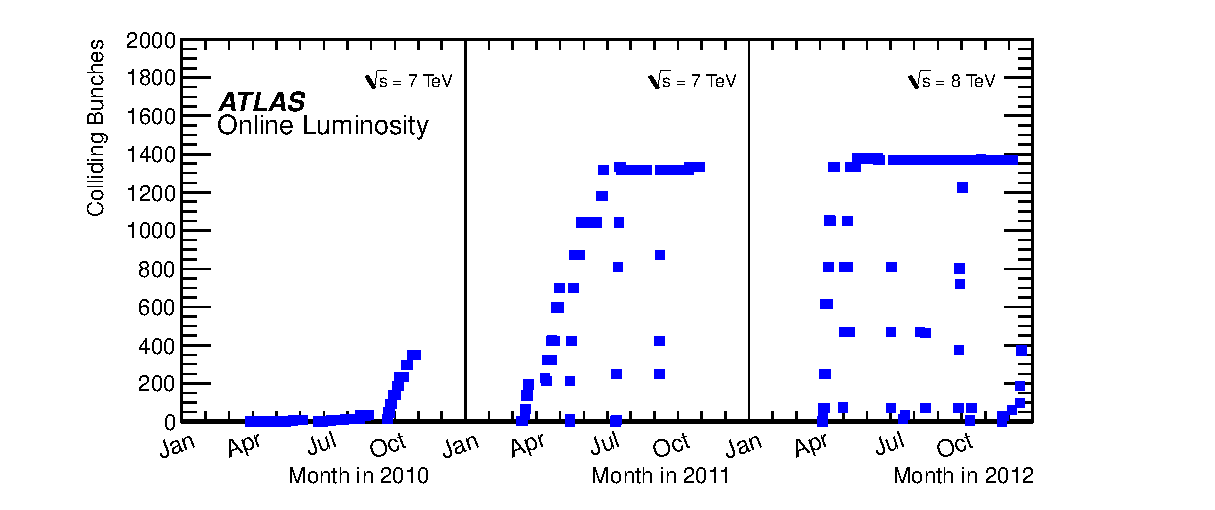
\includegraphics[width=\textwidth]{PartDetector/Plots/BunchesCollidingPerTime.eps}
      \caption{The number of bunches colliding per unit time at the LHC for the 2010, 2011 and 2012 $pp$ collision periods.}
      \label{fig:DetectorBunchesColliding}
    \end{subfigure}
  
    \begin{subfigure}[b]{0.95\textwidth}
      \includegraphics[width=\textwidth]{PartDetector/Plots/PeakLuminosityVsTime.eps}
      \caption{The peak luminosity per unit time at the LHC for the 2010, 2011 and 2012 $pp$ collision periods~\cite{Detector:LuminosityResults}.}
      \label{fig:DetectorPeakLumi}
    \end{subfigure}
    \caption{Shown in~\subref{fig:DetectorBunchesColliding} is the number of bunches colliding at the LHC and \subref{fig:DetectorPeakLumi} the peak luminosity per unit time.}
  \label{fig:DetectorPerformance}
\end{figure}

The acceleration of the proton beams occurs in several stages, within several different accelerators. The beams are first accelerated in a linear collider (LINAC 2) to an energy of \SI{50}{\MeV} before being injected into the proton synchrotron booster (PSB). The beams are then boosted to \SI{1.4}{\GeV} by a varying magnetic field in the circular PSB. The beams are then passed into the proton synchrotron (PS) and then the super proton synchrotron (SPS) where the beam energy increases to \SI{26}{\GeV} and then \SI{450}{\GeV}. At this stage the beam is injected into the LHC and then accelerated to the final desired energy. The design energy is \SI{7}{\TeV} per beam for a total of \SI{14}{\GeV} centre-of-mass energy. From injection of the protons into LINAC 2 to stable beam conditions in the LHC, the whole process can take a couple of hours.

As bunches overlap the protons that make up the bunches interact, these interactions are known as events. The number of events is proportional to the instantaneous luminosity $\Lagr$ of the collider. $\Lagr$ is a measure of the flux of particles per unit area per unit time can be defined as:

\begin{equation}
  \Lagr=fn_{b}\frac{N_1 N_2}{A}
\end{equation}
%
where $f$ is the frequency of revolution of the beam, $n_b$ the number of colliding pairs of bunches in the beam, $N_1$ and $N_2$ are the number of particles in each colliding bunch and A is the cross section of the beam~\cite{Luminosity}. The peak luminosity evolution at the LHC is shown in Figure~\ref{fig:DetectorPeakLumi}. Note that the operational $\sqrt{s}$ of the LHC was \SI{7}{\TeV} for 2010/11 and \SI{8}{\TeV} for 2012.

The total amount of data collected is measured by the integrated luminosity $\Lagr_{\textrm{int}}$ defined as the time integral of $\Lagr$. Integrated luminosity has units of inverse area, usually expressed in terms of barns (\si{\barn})\footnote{\SI{1}{\per\barn}=\SI{e-28}{\per\square\meter}}. The probability for a given process to occur is expressed as the cross section $\sigma$ and the total number of events which proceed via said process is defined as:
%
\begin{equation}
  \sigma\int\Lagr \dd t
\end{equation}

The integrated luminosity delivered by the LHC and collected by the ATLAS detector in 2011 and 2012 is shown in Figure~\ref{fig:DetectorIntLumi}. The ATLAS detector does not record all data delivered by the LHC; approximately $6.5\%$ was not recorded.

\begin{figure}[htbp]
  \centering
    \includegraphics[width=0.65\textwidth]{PartDetector/Plots/IntegratedLuminosity20112012.eps}
    \caption{Distribution of the total integrated luminosity delivered by the LHC and the recorded by ATLAS for the 2011 and 2012 $pp$ collision period. Note the $\sqrt{s}$ changing from \SI{7}{\TeV} to \SI{8}{\TeV} between 2011 and 2012~\cite{Detector:LuminosityResults}.} \label{fig:DetectorIntLumi}
\end{figure}

\subsection{Pileup}

Due to the large number of interactions and the short time between collisions, multiple events can overlap into a single event. This has detrimental effects on physics analyses and is a determining factor in setting the instantaneous luminosity with which to perform data collection. This overlapping effect is collectively known as pileup and is categorized into two types: in-time pileup, where multiple $pp$ collisions occur during the same bunch crossing; and out-of-time pileup, where the electric signals produced by previous collisions still remain to be read-out. This occurs when the time spacing between interactions is smaller than the read-out speed of the electronics. The number of interactions per crossing $\mu$ is shown in Figure~\ref{fig:DetectorBunchCrossingInteractions}, note that on average approximately thirty interactions occurred per bunch crossing in 2012. In comparison, in 2011 the average interactions per bunch crossing $\langle\mu\rangle$ varied from 5 in early 2011 to 15 at the end of the year.

\begin{figure}[htbp]
  \centering
    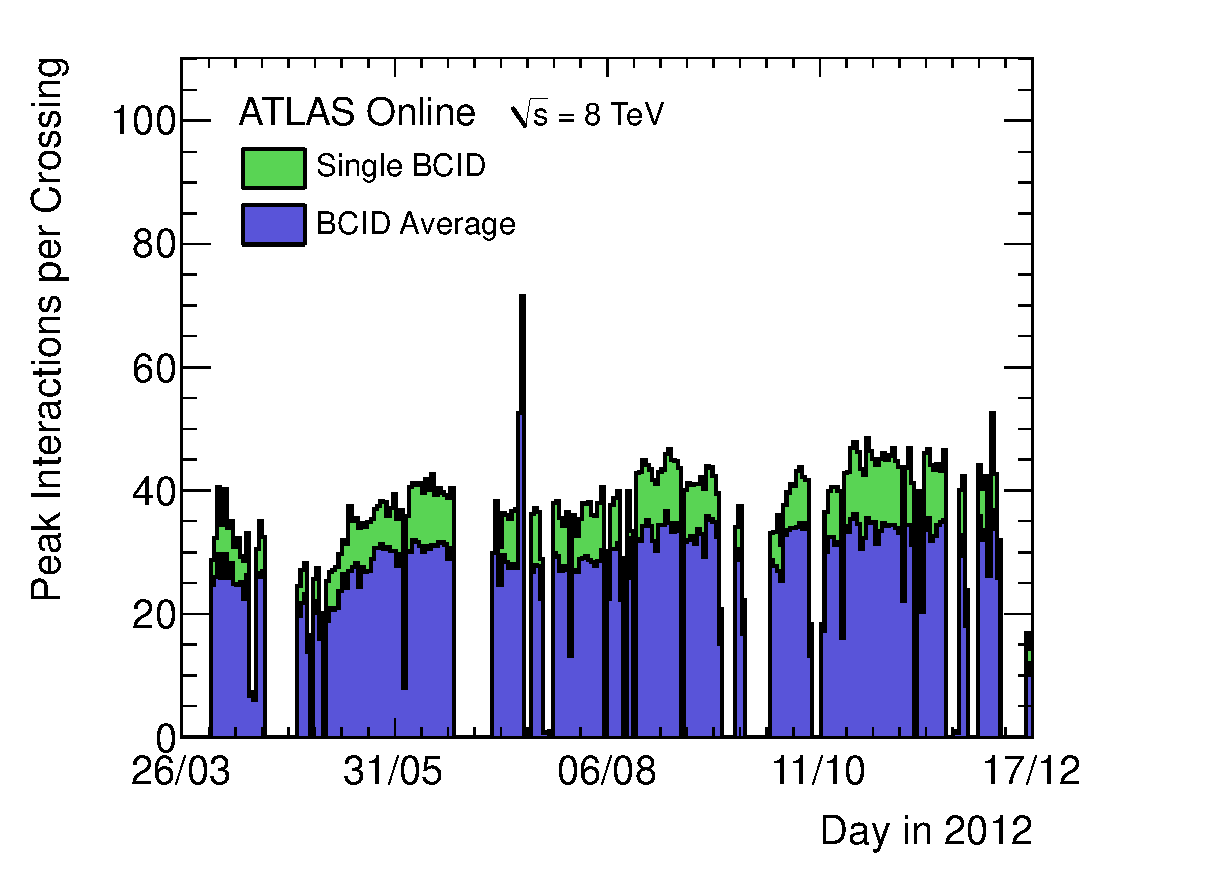
\includegraphics[width=0.65\textwidth]{PartDetector/Plots/peakBothMuByDay.eps}
    \caption{Number of interactions per bunch for the 2012 $pp$ data-taking period at ATLAS per day. Both the average number of interactions for all bunches and the maximum number of interactions are shown~\cite{Detector:LuminosityResults}.}
  \label{fig:DetectorBunchCrossingInteractions}
\end{figure}

\section{The ATLAS detector} \label{sec:the_atlas_detector}

The ATLAS~\cite{Detector:ATLASExperimentGeneral} experiment is a general-purpose detector which wraps around the IP providing large angular coverage. ATLAS is approximately cylindrical with a diameter of \SI{25}{\meter}, a total length of \SI{44}{\meter} and weighs \SI{7000}{\tonne}. The detector is made of several layers of instrumentation located at successively increasing radii as shown in Figure~\ref{fig:ATLASOverviewFigure}:

\begin{enumerate}
  \item \textbf{Inner Detector}: Located nearest to the beam-pipe and designed to measure the track of charged-particles.
  \item \textbf{EM Calorimeter}: Used for identification and measurement of electrons and photons.
  \item \textbf{Hadronic Calorimeter}: Used for the measurement of hadronic activity from hadronizing partons and missing transverse energy.
  \item \textbf{Muon Spectrometer}: The outermost detection layer, used for muon identification and measurement.
\end{enumerate}

Between these detection layers are magnets responsible for bending the path of the charged particles for the purpose of momentum measurement and particle identification. Additionally triggering and data acquisition (DAQ) systems form part of the detector for the purposes of recording the data signals coming from the aforementioned tracking and measurement systems. A brief description of these systems is provided in the coming sections. For a more detailed technical description of the detector and all subsystems see~\cite{Detector:ATLAS_TDR_vol1}.

Lepton plus jets \ttbar\ events produce a final state that includes hadronic activity, electrons, muons and missing energy and thus all elements of the detector are used in the reconstruction of such events. Additionally the match \xsm\ tagger which is central to this thesis, relies on the reconstruction and fitting of ID tracks and MS tracks. A detailed description of this algorithm is provided in Section~\ref{sec:DetectorSTACO}.

\begin{figure}[htbp]
  \centering
    \includegraphics[width=0.85\textwidth]{PartDetector/Diagrams/ATLAS_Overall.eps}
    \caption{An overview diagram of the ATLAS experiment. Shown are all detection and tracking systems and the toroid magnet which encompasses them. Note also the muon system on the outside of the detector.}
  \label{fig:ATLASOverviewFigure}
\end{figure}

A cylindrical coordinate system as used by all ATLAS publications has been adopted here. The coordinate system is constructed so that the $z$-axis is parallel to the beam axis. The $x$-axis is positive in the direction going from the IP to the centre of the LHC ring, and the positive $y$-axis points upwards. Thus the $x$-$y$ plane is transverse to the beam direction. All transverse variables such as the transverse momentum \pt, transverse energy \Et\ and missing transverse energy \met\ are measured along this plane. The azimuthal angle $\phi$ is measured around the beam axis, and the polar angle $\theta$ is the angle from the beam axis. The pseudorapidity is defined as $\eta=-\ln\tan(\theta/2)$. The distance in the $\eta$-$\phi$ plane between two objects is denoted by $\Delta R$ and defined as $\Delta R = \sqrt{\Delta\eta^{2}+\Delta\phi^{2}}$. Finally side A of the detector is defined as the positive $z$ side and side C is the negative $z$. Finally, the distance perpendicular to the beam-pipe is denoted by $R$. The transverse impact parameters $d_{0}$ is defined as the distance of closest approach (perigee) of a track to the primary vertex. The longitudinal impact parameter $z_{0}$ is the distance in $z$ between the perigee and the primary vertex.

\subsection{Inner Detector} \label{subsec:DetectorID}
The inner detector (ID) (Figure~\ref{fig:DetectorIDOverview}) is a tracking detector located closest to the beam-pipe and used for momentum and impact parameter measurement, vertex and track reconstruction and particle identification. The ID is designed to provide hermetic, high-resolution tracking in the range $\aeta<2.5$.

\begin{figure}[htbp]
  \centering
    \includegraphics[width=0.65\textwidth]{PartDetector/Diagrams/ATLAS_ID.eps}
    \caption{Drawing of the ATLAS inner detector.}
  \label{fig:DetectorIDOverview}
\end{figure}

The entire ID is contained within the central solenoid (CS) that generates a \SI{2}{\tesla} magnetic field for the purpose of momentum measurement. The trajectory of a charged particle is bent in the presence of a magnetic field by an amount proportional to the momentum of the particle
%
\begin{equation}
  r=\frac{\pt}{qB}
\end{equation}
%
where $r$ is the bending radius, \pt\ and $q$ are the transverse mass and charge of the particle, respectively, and $B$ is the magnetic field strength. The reconstruction of the path allows a measurement of the momentum. A particle with larger \pt\ would have a more straight trajectory than a low-\pt\ particle in the same magnetic field. For a central track with $\pt=\SI{5}{\GeV}$ the relative resolution on the measured transverse momentum is $\sim\SI{1.5}{\percent}$~\cite{Detector:ATLASExperimentGeneral}.

The reconstruction of interaction vertices is of paramount importance, particularly when considering the large amount of pile-up observed at ATLAS. Interaction vertices are reconstructed by fitting all reconstructed tracks to a point. The primary vertex (PV) is then defined as the vertex with the largest amount of momentum associated with it. In addition the reconstruction of secondary interaction vertices is used for the identification of short-lived particles such as $b$-hadrons and $\tau$.

\begin{figure}[htbp]
  \centering
  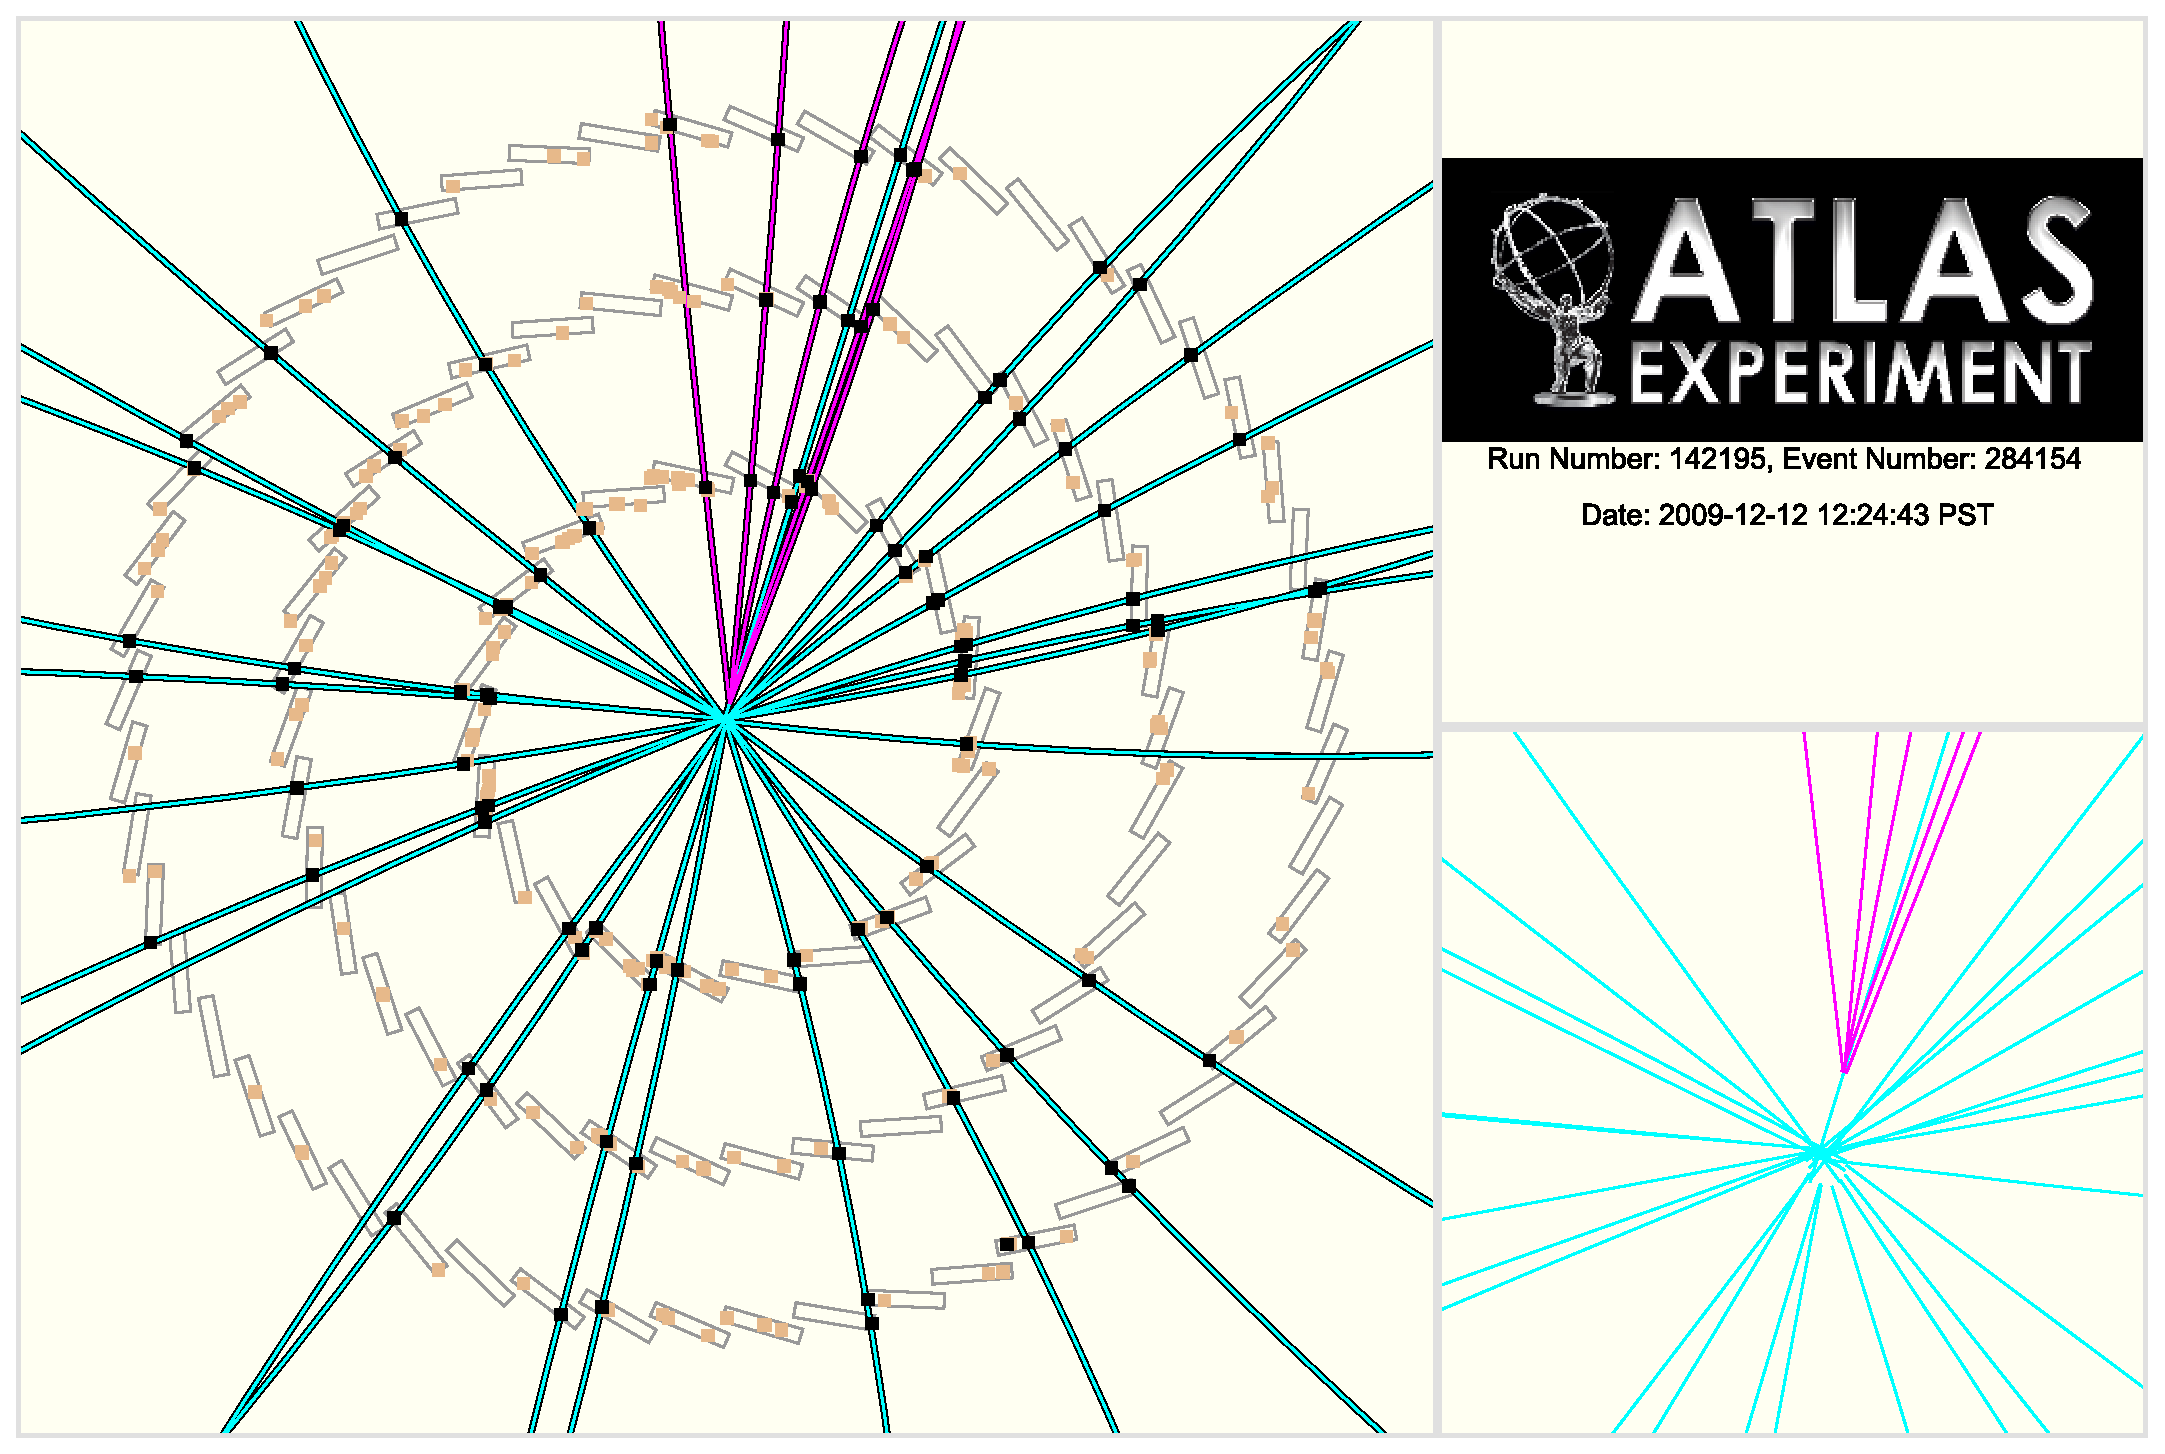
\includegraphics[width=0.75\textwidth]{PartDetector/Diagrams/fig_14.eps}
  \caption{An event-display of an event as reconstructed by the ATLAS inner detector. Shown are the results of the vertexing algorithm where each line represents a track. the purple tracks have been fitted to a secondary vertex.}
  \label{fig:DetectorEventDisplayID}
\end{figure}

The ID is made of three separate tracking and detection systems located at increasing radii away from the beam-pipe, the full arrangement can be seen in Figure~\ref{fig:DetectorIDQuarter} and a plane-view is shown in Figure~\ref{fig:DetectorIDTransverse}.

\begin{figure}[htbp]
  \begin{subfigure}[b]{0.45\textwidth}
    \centering
      \includegraphics[width=\textwidth]{PartDetector/Diagrams/Detector_ID_QuarterView.eps}
      \caption{Plan-view of a quarter-section of the ATLAS ID showing the major detector elements with its active dimensions and envelopes. Note also the $\eta$ markers showing the maximum coverage up to $\eta=2.5$~\cite{Detector:ATLASExperimentGeneral}.}
    \label{fig:DetectorIDQuarter}
  \end{subfigure}
  \hfill
  \begin{subfigure}[b]{0.45\textwidth}
    \centering
      \includegraphics[width=\textwidth]{PartDetector/Diagrams/ID_3D_Overview.eps}
      \caption{A drawing of in the transverse plane of the ATLAS ID showing all major detection elements in the barrel regions~\cite{Detector:ATLASExperimentGeneral}. A charged particle track is shown traversing all the detector elements as a solid line.}
    \label{fig:DetectorIDTransverse}
  \end{subfigure}
\end{figure}



\subsubsection{Pixel detector}

The pixel detector is located nearest to the beam-pipe and provides high-granularity and precision for secondary vertex reconsruction. As a charged particle passes through a sillicon pixel, an electron-hole pair is created. The electron and hole begin drifting in opposite directions under the influence of a voltage and the charge is then read out through an electrode. This signal is read out as a \emph{hit} by read-out electronics. The pixel detector consists of three silicon pixel sensor layers in the barrel region located at approximately \SIlist{5;9;12}{\cm} from the IP, and three disks at each side located at constant $R$ providing coverage up to $\aeta<2.5$. The barrel modules are overlapped in a turbine pattern to provide hermetic coverage. In the barrel region the modules provide an intrinsic resolution of \SI{10}{\um} in \rphi\ and \SI{115}{\um} in $z$~\cite{Detector:ATLASExperimentGeneral}. The disk sections have an intrinsic resolution of \SI{10}{\um} (\rphi) and \SI{115}{\um} ($R$).

\subsubsection{Semiconductor tracker}
The semiconductor tracker (SCT) located in the intermediate radius range is designed to provide eight hits per track contributing to the measurement of momentum, impact parameter and vertex position. The SCT is made of four layers of stereo-pair silicon micro-strip sensors in the barrel region at increasing radii with an intrinsic resolution of \SI{17}{\um} (\rphi) and \SI{580}{\um} ($z$). At the end-caps nine disks of silicon microstrip modules provide large $\eta$ coverage with a resolution of \SI{17}{\um} (\rphi) and \SI{580}{\um} ($R$)~\cite{Detector:ATLASExperimentGeneral}.

\subsubsection{Transition radiation tracker}
The transition radiation tracker (TRT) is the outermost tracking layer that forms the ID and it acts as both a tracker and transition radition detector. Transition radiation (TR) is produced when a charged particle crosses the boundaries of two materials with different dielectric constants. The probability of producing TR photons depends on the Lorentz factor of the particle $\gamma=E/m$. Thus for two particles of the same energy, a lighter particle will on average emit more ionization than a heavier particle.

The TRT is designed to provide up to \num{36} hits per track using straw-tube sensors. Each straw is \SI{4}{\mm} in diameter and is made of two \SI{35}{\micro\meter} thick Kapton multi-layer films bonded back-to-back. At the center of each straw is a gold plated tungsten wire with a diameter of \SI{31}{\micro\meter} and the straw is filled with a mixture of gas (\SI{70}{\percent} xenon, \SI{27}{\percent} $\textrm{CO}_{2}$ and \SI{3}{\percent} $\textrm{O}_2$). The tubes are surrounded by polypropylene-polyethylene fibers that act as radiators and allow for the production of TR, which later ionizes the gas mixutre and is read-out through the gold-plated wire.

In the barrel the \SI{144}{\cm} long straw-tubes are arranged in modules which contain between \num{329} and \num{793} straws. The end-cap disks are made of radially distributed \SI{36}{\cm} long straw-tubes. Each straw-tube provides an intrinsic resolution of \SI{130}{\um} along its length~\cite{Detector:ATLASExperimentGeneral}. The combination of a large number of hits over a large radius allows measurements in the TRT to be made with an accuracy that can complement those made by the pixel detector.

\subsection{Calorimetry}
The ATLAS calorimeter is responsible for the measurement of the energy of particles that emerge from the event. Sampling calorimeters are used for this purpose, layers of absorber material (passive) are placed in the path of the particles forcing them to interact and shower. The amount of energy lost by the incident particle depends on the type of material the particle traverses, the energy of the particle and the type. At high energies electrons lose energy predominantly via Bremsstrahlung, while photons lose energy via pair production. The characteristic length associated with this energy loss is a material characteristic known as the radiation length $X_0$.

For electrons the energy as a function of material traversed is 
%
\begin{equation}
  E=E_0e^{-x/X_0}
\end{equation}
%
where $E$ is the energy of the incident particle, $E_0$ is the initial energy and $x$ is the distance traversed. As an electron traverses one $X_0$ of material, its energy is reduced by a factor of $1/e$. For photons the average number of photons traversing through a material length $x$ is reduced exponentially by a factor of $\frac{7}{9}X_0$. Thus the longitudinal length of the shower is proportional to the logarithm of the energy of the incoming particle.

The number of shower particles changes as a function of the interaction length $\lambda_{\textrm{int}}$ as
%
\begin{equation}
  N=N_{0}e^{-x/\lambda_{\textrm{int}}}
\end{equation}
%
where $N$ is the number of shower particles at length $x$ and $N_{0}$ is the initial number of incident particles. This is the characteristic length used when discussing the construction of the hadronic calorimeter. For a given material the $\lambda_{\textrm{int}}$ is much larger than $X_{0}$ and thus therefore hadronic showers tend to be much broader and deeper than EM showers. Note that on average $1/3$ of the particle content of a hadronic showers is EM mostly due to pion decay into photons.

The energy of the resulting shower is then measured by some sampling material (active) located behind the absorbers, this energy is proportional to the energy of the incident particle.

The type and thickness of material used is varied through the pseudorapidity range to improve energy measurement and reduce punch-through of particles into the muon systems behind. Due to the large amount of intense radiation produced during collisions, radiation hardness is also a driving factor in material choice.

The ATLAS calorimeter consists of the EM calorimeter, designed to measure photons and electrons covering the pseudorapidity region $\aeta<3.2$; the hadronic calorimeter (HCal), which measures hadronic activity covering the pseudorapidity region $\aeta<3.2$; and the forward calorimeter (FCal) which provides energy measurement capability in the very high pseudorapidity region $3.1<\aeta<4.9$. As can be seen in Figure~\ref{fig:ATLASCalorimetryOverall} the calorimetry envelopes the ID and CS providing hermetic coverage symmetric in $\phi$. This is particularly important for the measurement of \met\ resulting from weakly interacting particles escaping the detector.

\begin{figure}[htbp]
  \centering
  \includegraphics[width=0.75\textwidth]{PartDetector/Diagrams/ATLAS_Calorimetry.eps}
  \caption{A cut-away diagram of the ATLAS detector highlighting the calorimetry system. Shown are the ECal barrel and end-cap, the HCal barrel and end-cap and the FCal end-cap~\cite{Detector:ATLASExperimentGeneral}.}
  \label{fig:ATLASCalorimetryOverall}
\end{figure}

\subsubsection{Electromagnetic calorimeter}
The EM calorimeter is made of a barrel section ($\aeta<1.475$) and two end-caps ($1.375<\aeta<3.2$). The EM barrel consists of two half-barrels separated by a \SI{4}{\mm} gap at $z=0$. The end-caps consist of two coaxial wheels, the outer ring covering the pseudorapidity range $1.375<\aeta<2.5$ and the inner ring covering the range $2.5<\aeta<3.2$. The pseudorapidity region $1.37<\aeta<1.52$ is not used for precision physics due to the large amount of material, this is known as the ``crack'' region.

The EM calorimeter employs liquid Argon (LAr) as the active material due to its intrinsic radiation hardness and response over time, and lead as the passive material arranged in an accordion geometry for full $\phi$ symmetry. Particles interact with the lead absorbers creating a shower which ionizes the layers of liquid Argon. A potential is applied across the LAr material allowing for signal readout via Kapton/copper electrodes. The total thickness of the EM calorimeter is $>24X_{0}$ in the barrel and $>26X_{0}$ in the end-caps. The amount of material is optimized in pseudorapidity to enhance energy resolution.

In the region devoted to precision physics the EM calorimeter is divided into three segments as shown in Figure~\ref{fig:DetectorECalSegment}, the strip layer is designed to improve particle identification and pseudorapidity position measurement. The design energy resolution for all components of the calorimeter are shown in Table~\ref{tab:DetectorCaloResolution}.

\begin{table}
  \ra{1.3}
  \centering
  \begin{tabular}{@{}ll@{}}
    \toprule
    Section   & Resolution \\
    \midrule
    EM Barrel & $\frac{10.1\%}{\sqrt{E}}\oplus0.17\%$~\cite{Energy} \\
    EMEC      & $\frac{10\%}{\sqrt{E}}\oplus0.7\%$ \\
    HEC       & $\frac{100\%}{\sqrt{E}}\oplus10\%$ \\
    FCAL      & $\frac{100\%}{\sqrt{E}}\oplus10\%$ \\
    % EM Barrel & $\frac{10\%}{\sqrt{E}}\oplus0.7\%$
    % HEC       & $\frac{70.6\%}{\sqrt{E}}\oplus5.8\%$ \\ MEASURED
    % FCAL      & $\frac{95\%}{\sqrt{E}}\oplus7.5\%$~\cite{Detector:FCalMeasuredPerf} \\ MEASURED
    \bottomrule
  \end{tabular}
  \caption{Design energy resolution of all ATLAS calorimeter components. The resolution is made of a sampling term ($\nicefrac{1}{\sqrt{E}}$) associated with the choice of passive and active materials and the construction of the layers, and a constant term associated with the depth of the detector, cracks and dead material.} \label{tab:DetectorCaloResolution}
\end{table}

\begin{figure}[htbp]
   \centering
   \includegraphics[width=0.75\textwidth]{PartDetector/Diagrams/LARG3-TDR-barrelM.pdf}
   \caption{Cut-away diagram of the EM calorimeter barrel at $\eta=0$. Shown are the three different layers with varying cell structures. The strip section is designed to enhance particle identification and position measurement in $\eta$.}
   \label{fig:DetectorECalSegment}
 \end{figure} 

\subsubsection{Hadronic calorimeter}
The hadronic calorimeter uses different types of passive and active material to accommodate for the varying conditions in different regions of the detector. The materials used and structure of the detector must provide good energy resolution, full symmetric coverage for the purpose of \met\ measurement, full containment of all hardonic activity to prevent punch-through to the muon system and be sufficiently radiation hard.

The hadronic calorimeter consists of two parts a scintillator tile calorimeter in the barrel region, and a LAr calorimeter in the end-cap.

The tile calorimeter is located directly outside the EM calorimeter. The barrel portion of the calorimeter covers the region $\aeta<1.0$ and the two extended barrels cover the range $0.8<\aeta<1.7$. The tile calorimeter uses steel as the passive material and scintillating tiles as the active material. The resulting hadronic showers enter the scintillating tiles and produce photons which are passed to photomultiplier tubes. The total detector thickness which is tile-instrumented is $9.7\lambda_{\textrm{int}}$ at $\eta=0$.

The hadronic end-cap (HEC) uses LAr technology due to its radiation-hardness in this challenging high pseudorapidity region. The HEC consists of two independent wheels per end-cap covering the range $1.5<\aeta<3.2$ overlapping the tile calorimeter at low pseudorapidity range and the forward calorimeter located at high pseudorapidity.

\subsubsection{Forward calorimeter}

The forward calorimeter (FCal) is responsible for energy measurement in the very-high pseudorapidity range $3.1<\aeta<4.9$ of both electromagnetic and hadronic activity. Due to the large amount of radiation in this region, LAr is employed as the active material. The FCal consists of three layers, the first made primarily of copper, designed mostly for the measurement of electromagnetic activity while the two outer tungsten layers are responsible for hadronic activity measurement.

\subsection{Muon spectrometer}

The muon spectrometer (MS) is the outer most layer of the ATLAS detector (Figure~\ref{fig:DetectorDrawingMuonSystem}) and is responsible for the precision measurement of \pt\ of charged-particles that pass-through the ATLAS calorimetry. It is designed to detect charge particles leaving the calorimeters and measure their momentum with a precision of \SI{10}{\percent} at a momentum of \SI{1}{\TeV}~\cite{Detector:ATLASExperimentGeneral}. Muon tracking performance is vital to the SMT tagger described in Section~\ref{sec:DetectorSLT}, as it relies on the precise reconstruction of muon tracks in the ID and MS. Inner detector tracks and Muon spectrometer tracks are fitted to form a \emph{combined} muon track, the quality of the fit is at the core of the SMT algorithm.

Due to their larger mass, muons tend to have a larger transverse momentum and as such do not lose as much energy through the emission of photons in the calorimetry. As a result, muons tend to traverse the hadronic calorimeter and escape the detector volume. The muon system provides measurement of these particles up to $\aeta<2.7$ and triggering up to $\aeta<2.4$. Measurement of \pt\ is facilitated by the magnetic field generated by the large toroid magnet in the barrel region $\aeta<1.4$ and two smaller end-cap magnets in $1.6<\aeta<2.7$. In the transition region ($1.4<\aeta<1.6$) deflection is provided by the barrel and end-cap fields. 

\begin{figure}[htbp]
  \centering  
  \includegraphics[width=0.95\textwidth]{PartDetector/Diagrams/ATLAS_MuonSystem.eps}
  \caption{Cut-away drawing of the ATLAS muon system.}
  \label{fig:DetectorDrawingMuonSystem}
\end{figure}

The structure of the MS is delimited by the magnet system. In the barrel region three cylindrical layers of precision-tracking chambers are located in and on the coils of the barrel toroid magnet at radii of ~\SIlist{5;7.5;10}{\meter}. End-cap region coverage is provided by three chamber planes perpendicular to the $z$-axis located in front and behind the end-cap toroid magnet at distances $|z|\approx$~\SIlist{7.4;10.8;14;21.5}{\meter} from the interaction point.

The MS contains four different types of chambers responsible for precision-tracking and/or triggering in various pseudorapidity ranges as shown in Table~\ref{tab:DetectorMSOverview}. The arrangement of these chambers is shown in Figure~\ref{fig:DetectorMuonOverview}. 

\begin{table}
  \centering
  \begin{tabular}{@{}ll@{}}
    \toprule
    \textbf{Monitored drift tubes} & \textbf{MDT} \\
    \midrule
    - Coverage                     & $\aeta<2.7$ (innermost layer: $\aeta<2.0$) \\
    - Number of chambers           & 1150 \\
    - Function                     & Precision tracking \\
    \bottomrule
    \textbf{Cathode strip chambers} & \textbf{CSC} \\
    \midrule
    - Coverage                      & $2.0<\aeta<2.7$ \\
    - Number of chambers            & 32 \\
    - Function                      & Precision tracking \\
    \bottomrule
    \textbf{Resistive place chambers} & \textbf{RPC} \\
    \midrule
    - Coverage                        & $\aeta<1.05$ \\
    - Number of chambers              & 606 \\ 
    - Function                        & Triggering, second coordinate \\
    \bottomrule
    \textbf{Thin gap chambers}        & \textbf{TGC} \\
    \midrule
    - Coverage                        & $1.05<\aeta<2.7$~(2.4 for triggering) \\
    - Number of chambers              & 3588 \\
    - Function                        & Triggering, second coordinate \\
    \bottomrule
  \end{tabular}
  \caption{Main parameters of the muon system~\cite{Detector:ATLASExperimentGeneral}.}
  \label{tab:DetectorMSOverview}
\end{table}

\begin{figure}[tbhp]
  \centering
  \begin{minipage}[b]{0.47\textwidth}
    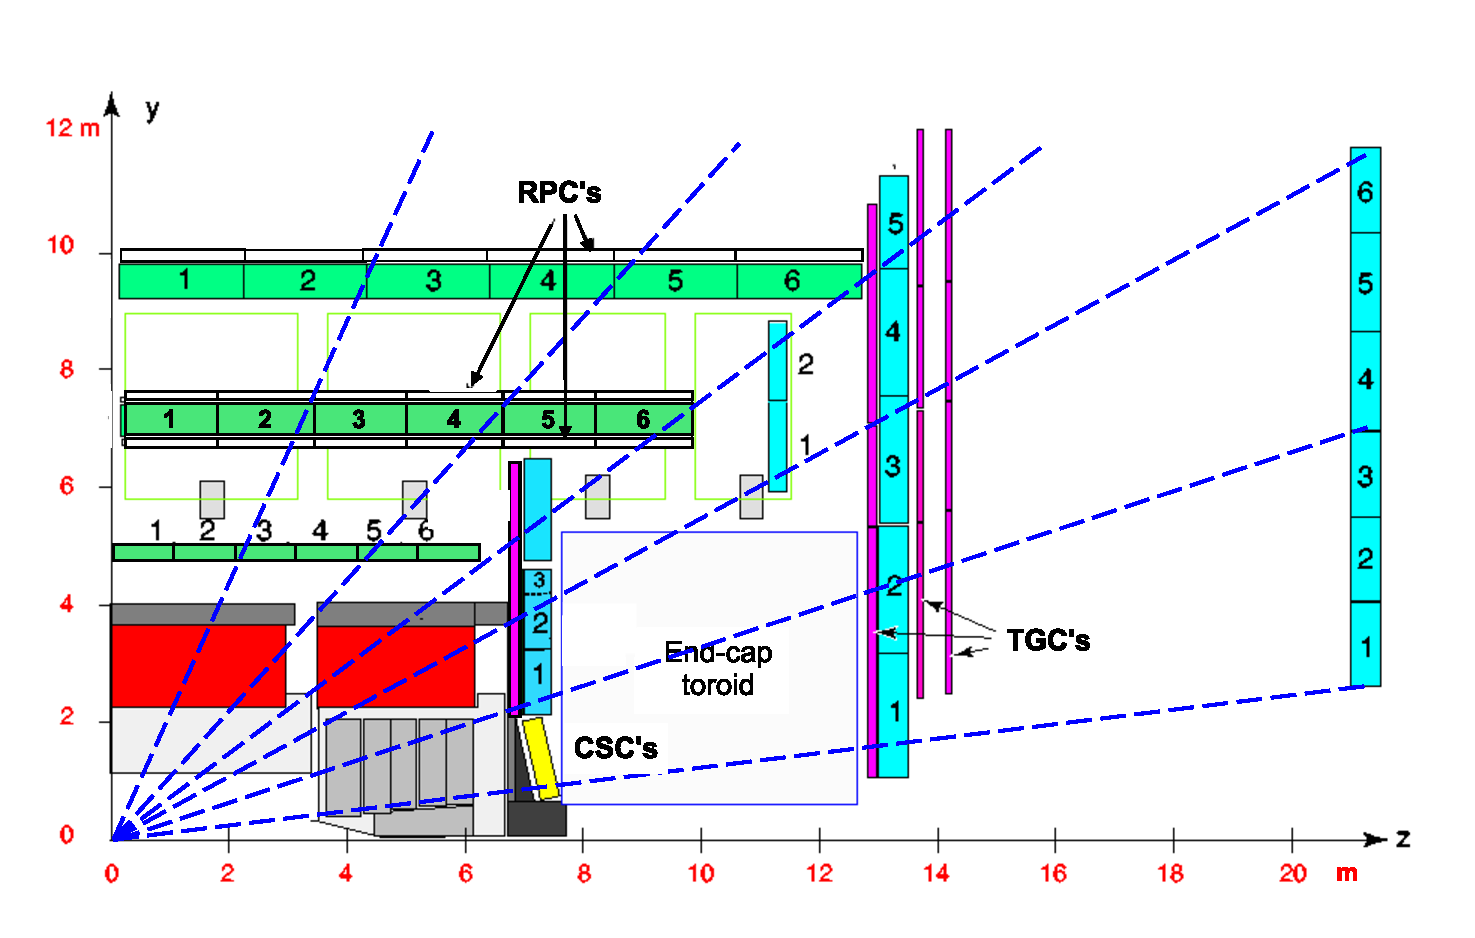
\includegraphics[width=\textwidth]{PartDetector/Diagrams/Muon_section.eps}
  \caption{Plan view of quarter-section of the ATLAS muon spectrometer.} \label{fig:DetectorMuonOverview}
  \end{minipage}
  \hfill
  \begin{minipage}[b]{0.47\textwidth}
   \includegraphics[width=\textwidth]{PartDetector/Diagrams/Muon_sector_numbering.pdf}
  \caption{Transverse view of the muon system. Shown are the } \label{fig:DetectorTransverse}
  \end{minipage}
\end{figure}

In the barrel region, precision-measurement is performed by monitored drift tubes (MDT) chambers. These chamber consist of three to eight pressurized aluminium drift tubes, each containing a tungsten-rhenium wire anode and a mixture of argon and carbon dioxide gas. An average spatial resolution of \SI{80}{\um} per tube and \SI{35}{\um} per chamber is achieved.

The end-cap region is instrumented with cathode-strip chambers (CSC) due to their higher rate capability and time resolution. CSCs are multiwire chambers with cathode planes segmented into strips in orthogonal directions. This allows both coordinates to be measured simultaneously. The resolution of a chamber is \SI{40}{\um} in the bending plane ($R$-$z$) and \SI{5}{\mm} in the transverse plane.

Triggering on muon tracks is another essential role of the muon spectrometer. To this end, each precision-measurement chamber is complemented with fast triggering chambers. As with the measurement layers, two different types of chambers are used for the barrel and end-cap regions. In the barrel region ($|\eta<1.05$) resistive plate chambers (RPC) are used attached to the same support structure as the MDTs. The RPCs are made of two resistive plates, \SI{2}{\mm} apart, between which a potential difference is applied. The gap between the plates is filled with a mixture of $\textrm{C}_2\textrm{H}_2\textrm{F}_4$/Iso-$\textrm{C}_4\textrm{H}_{10}$/$\textrm{SF}_6$. The signal is read out via metallic strips mounted to the outer faces of the resistive plates. The end-cap region ($1.05<\aeta<2.4$) is populated with thin gap chambers (TGC). TGCs multiwire chambers like those used in the CSC, however the distance between the wire and the cathode is smaller in the TGC. A summary of the spatial and temporal resolution for the measurement and triggering layers is shown in Table~\ref{tab:MSPerfomanceSummary}.
%
\begin{table}
  \centering
  \begin{tabular}{@{}lccc@{}}
   \toprule
   Chamber & \multicolumn{3}{c}{Resolution in} \\
   \cmidrule{2-4}
           & $R/z$ & $\phi$ & Time \\
   \midrule
   MDT & \SI{35}{\um} $(z)$ & -- & -- \\
   CSC & \SI{40}{\um} $(R)$ & \SI{5}{\mm} & \SI{7}{\ns} \\
   RPC & \SI{10}{\mm} $(z)$ & \SI{10}{\mm} & \SI{1.5}{\ns} \\ 
   TGC & \SIrange[range-phrase=-,range-units=single]{2}{6}{\mm} $(R)$ & \SIrange[range-phrase=-,range-units=single]{3}{7}{\mm} & \SI{4}{\ns} \\
   \bottomrule
  \end{tabular}
  \caption{Summary of spatial and temporal resolutions per chamber for all chamber types used in the ATLAS muon spectrometer. Adapted from~\cite{Detector:ATLASExperimentGeneral}.}
  \label{tab:MSPerfomanceSummary}
\end{table}

\subsection{Magnet system}
The structure of the ATLAS detector is defined by the large magnet system. The ATLAS magnet system, shown in Figure~\ref{fig:DetectorMagnet}, consists two sets of magnets. The central solenoid and three air-core toroids.

The central solenoid located nearest to the beam, provides a \SI{2}{\tesla} magnetic field for the ID for the purpose of tracking, particle identification and \pt\ measurement.

The barrel toroids extend to $\aeta<1.4$ and are made of eight coils, generating a \SI{0.5}{\tesla} magnetic field for the MS. In the high pseudorapidity range, magnetic deflection is provided by two end-cap toroids extending from $1.6<\aeta<2.4$. As in barrel, the end-cap toroids are made of eight coils offset by \SI{22.5}{\degree} with respect to the barrel coils. Each end-cap generates a \SI{1}{\tesla} magnetic field for the MS. The so-called transition region between the two magnets is covered by an overlap of the end-cap and barrel fields.

\begin{figure}[htbp]
  \centering
  \includegraphics[width=0.75\textwidth]{PartDetector/Diagrams/ATLcoilGeom.eps}
  \caption{Diagram of the ATLAS toroid magnet system. The red central solenoid is located closest to the beam surrounded by layers of tile calorimetry. The eight barrel toroid magnets are shown along with the offset end-cap toroids at each end.}
  \label{fig:DetectorMagnet}
\end{figure}

\subsection{Beam-pipe}

The beam-pipe section located within the ATLAS experiment is approximately \SI{38}{\meter} in length and made of seven parts. The central chamber has an inner diameter of \SI{58}{\mm} and is constructed from \SI{0.8}{\mm} thick beryllium due to the material's transparency to particles, high specific stiffness and compatibility with ultra-high vacuum. The beam-pipe is centred around the IP and integrated with the pixel detector. The additional layers are made of stainless steel located symmetrically on both sides of the IP.

\subsection{Triggering and DAQ}

At the design luminosity of the LHC $\Lagr=\SI{10e34}{\per\square\cm\per\second}$, the expected event rate is approximately \SI{1}{\GHz}. At an average event size of \SI{1.3}{\mega\byte} per event, the total amount of data produced at ATLAS is \SI{1.2}{\peta\byte\per\second}. The maximum rate of data storage at ATLAS is approximately \SI{300}{\mega\byte\per\second}, so the rate must be reduced.

The trigger and data acquisition system (TDAQ) is responsible for selecting only ``interesting'' events for recording, thus reducing the rate. This is known as an \emph{online selection} as it happens before the data is stored. Selections during analysis for example, are known as \emph{offline selection}, as they happen after the data has been recorded.

The overwhelming majority of events produced at the LHC are of no interest to physics analysis, for example the so-called \emph{minimum bias events}. 

At ATLAS, trigger decisions are carried out in three sequential levels: \emph{Level 1} (L1), \emph{Level 2} (L2) and \emph{Event Filer} (EF), each successive level reduces the rate by applying increasingly more complex selection criteria. The hardware-based L1 trigger, performs the initial selection based on reduced-granularity information from the MS trigger chambers and all calorimeters. Data from the calorimeter trigger towers, shown in Figure~\ref{fig:DetectorECalSegment}, is used to search for presence of high transverse-momentum muons, photons, electrons, hadronic decays of $\tau$ leptons and hadronic jets, as well as large missing transverse energy and large total transverse energy. The central trigger processor applies the the trigger `menu' which includes a combination of selection criteria. Events which are of interest to physics analyses can be produced at such a rate as to overwhelm the capabilities of the DAQ. A \emph{prescale} can be applied to record one out of many of these events, thus reducing the rate. The L1 trigger also constructs \emph{regions of interest} (RoIs) around the detector where interesting features have been found. The $\eta$ and $\phi$ information of the RoI along with information about the decision is stored and passed to the higher level triggers.

The L2 selection makes use of RoIs and the full granularity of the detector to further reduce the event rate to approximately \SI{3.5}{\kHz} and finally the EF implements selections commonly used for offline analysis to reduce the rate to \SI{200}{\Hz}.



\section{Monte Carlo Simulation} \label{DetectorMC}

The simulation of data is paramount to HEP research, from the initial detector design phase all the way through to finalized analyses. Monte Carlo (MC) generators simulate various interactions, creating kinematic collision event data that reflect our best understanding of nature. These processes are then passed through detector simulation and all the object reconstruction algorithms, resulting in a dataset with an identical format to collision data. More information on the ATLAS simulation infrastructure can be found in~\cite{Detector:ATLASSimulationInfra}.

The simulation of data happens in three phases: event generation, detector simulation and digitization. 

\subsection{Event Generation} \label{DetectorEventGeneration}

Event generators are tools that model complex physics processes that occur during a particle collision. Many different generators exist to model a variety of beam types ($pp$, $p\bar{p}$, $e^+e^-$, etc\ldots) and event types. Hadronic event generation simulates all components which make up the interaction, namely the hard scattering process, parton showering, hadronising, hadronic decay, the underlying event and photon radiation~\cite{Les} as shown in Figure~\ref{fig:DetectorEGSketch}.

\begin{figure}[htbp]
  \centering
  \includegraphics[width=0.85\textwidth]{PartDetector/Diagrams/scetch.eps}
  \caption{Sketch of a proton-proton collision as modelled by the event generator~\cite{Event}. Shown are the incoming protons beams as green arrows on the left and right sides of the diagram. The partons shown in blue, interact in the hard interaction (red blob) producing a parton shower, also depicted in red, which eventually hadronize (light green blobs) and finally decay into final state particles shown in dark green. The \emph{underlying event} is shown at the bottom of the diagram as the purple blob, note also the beam remnants as light blue blobs that also form part of the underlying event. Photon emission is shown in yellow and occurs at all stages of the event generation.}
  \label{fig:DetectorEGSketch}
\end{figure}

First, the \emph{hard interaction} of a pair of partons originating from the colliding protons is simulated. An example of such an interaction is $q\bar{q} \rightarrow Z / \gamma^{*}\rightarrow e^{+}e^{-}$. Calculating the cross section for such an interaction involves the convolution of the parton density function (PDF) and the \emph{matrix element} (ME).

The PDF $f_i(x,Q^2)$, describes the probability of finding, within the proton, a parton of flavour $i$ carrying a fraction $x$ of the proton momentum, via a hard interaction with energy scale $Q$. The ME describes the interaction between the two partons and corresponds to one or more of the Feynman diagrams associated with the interaction\footnote{For a rigorous discussion of matrix elements and the Feynman rules, see~\cite{Theory:Perkins,Theory:IntroGriffiths}}. The order of a diagram is determined by the number of coupling constants associated with it. Different generators are capable of treating diagrams at different orders. The hard interaction is usually modelled at LO or NLO.

The next step is \emph{parton-showering} which simulates the  emission of gluons by coloured partons. A cascade of partons is produced, as shown in Figure~\ref{fig:DetectorEGSketch}, and modelled by perturbation theory for energies above \SI{1}{GeV}. All coloured objects are then combined into colourless hadrons in a process known as \emph{hadronization}, these hadrons are subsequently allowed to decay.

Finally, the remaining coloured partons not involved in the hard interaction, are allowed to interact forming the \emph{underlying event}.

The kinematic information of the original event without the effects of the detector is kept in the data set and is usually referred to as the \emph{truth information}.

\subsection{Detector simulation} \label{sec:DetectorSimulation}

The generated events are then passed through a detector simulation that mimics the response of the detector to particles traversing through it. A description of the entire detector is implemented in the GEANT4 tool-kit~\cite{Detector:Geant4}, including a map of the magnetic fields, the position of the detector components and material description. The software then simulates the signal voltages produced in all tracking and calorimeter components of the detector, these are then passed through a simulation of the read-out electronics and DAQ taking into account known losses and inefficiencies. All of this information is then passed on to the reconstruction software that ``rebuilds'' the physics objects from the detector \emph{hits}.

\section{Object reconstruction} \label{sec:DetectorEventReco}

The process of converting the raw data from the detector into physics objects (electrons, muons and so on) is known as \emph{object reconstruction}. The algorithms for object reconstruction are identical for both collision data and simulated data. As lepton plus jets decays of \ttbar\ are the focus of this thesis, the reconstruction procedures of all types of objects (excluding photons) are relevant. This includes electron, muon and jet reconstruction as well as $b$-tagging algorithms. The focus of this thesis, the soft muon tagger, relies on \emph{STACO combined} muons, therefore some details of the muon reconstruction algorithms are discussed here.

\subsection{Electron reconstruction} \label{sec:DetectorElReco}

The electron reconstruction~\cite{Detector:ElectronReco} procedure at ATLAS depends on the pseudorapidity of the candidate. Only electrons that lie within the coverage of the ID are used here, therefore only the relevant procedure is described. The algorithm used in the central region identifies energy deposits in the EM calorimeter and associates them with reconstructed ID tracks. Firstly, clusters are seeded from energy deposits with total \Et\ above \SI{2.5}{\GeV} using a sliding-window algorithm with window size $3\times5$ in units of $0.025\times0.025$ in ($\eta$,$\phi$) space. Tracks with $\pt>\SI{0.5}{\GeV}$ are then extrapolated to the middle layer of the EM calorimeter and then matched to the cluster seed using cuts in the ($\eta$,$\phi$) space. In case of multiple matches, tracks with pixel or SCT hits are given priority and the match with the smallest \DeltaR\ distance is chosen. Finally, the size of the cluster associated with the candidate electron is enlarged to $3\times7$ and $5\times5$ in the barrel and endcap regions respectively. The energy of the electron is then the sum of four contributions taking into account energy deposited before the EM material, and leakages to other clusters or beyond the EM calorimeter. 

Electron identification for central electron cadidates is done by applying sequential cuts on calorimeter, tracking and combined track-cluster variables. Several sets of selection criteria, labelled \emph{loose}, \emph{medium} and \emph{tight}, are designed for use in analyses. These sets provide increasing background-rejection power at the cost of efficiency by introducing new cuts at each stage or by tightening previous cuts. The cut definitions are listed in Appendix~\ref{app:DetectorElectronID}.

Additional requirements can be made on the so-called isolation of the electron. Three sets of isolation strategies are used at ATLAS~\cite{Detector:ElectroIsolation}:

\begin{itemize}
  \item \textbf{Calorimeter isolation}: The calorimeter isolation \etcone{\DeltaR}\ is defined as the sum of transverse energy deposited in the cells around the electron in a cone of size \DeltaR. The contribution from the electron itself is removed within $\Delta\eta\times\Delta\phi=0.125\times0.175$ around the electron cluster barycenter. It is corrected for energy leakage from the electron into the isolation cone and for the effect of pile-up. At ATLAS the nominal cone sizes used are $\DeltaR$=\numlist{0.2;0.3;0.4}.
  \item \textbf{Track isolation}: The tracking isolation \nucone{\DeltaR}\ is defined as the number of tracks in a cone around the electron, excluding the track of the electron itself.
  \item \textbf{Momentum isolation}: The momentum isolation \ptcone{\DeltaR}\ is defined by the sum of the transverse momentum of tracks with $\pt>\SI{0.4}{\GeV}$ in a cone around the electron, excluding the electron track itself.
\end{itemize}

\subsection{Muon reconstruction} \label{sec:DetectorMuReco}

Muon reconstruction makes use of the information provided by both the inner detector and the muon spectrometer systems. Several different strategies exist~\cite{Detector:MuonReconstructionList}:

\begin{itemize}
  \item \textbf{Standalone reconstruction}: Uses MS information only, first constructing \emph{segments} from several hits in a given chamber and then fitting segments from all three stations to hits from the four MS components. Tracks are then extrapolated back to the IP taking into account energy loss and multiple scattering.
  \item \textbf{Tagging ID tracks reconstruction}: Uses MS or calorimeter information to tag ID tracks as muons.
  \item \textbf{Combined track reconstruction}: Standalone muon tracks are extrapolated back to the vertex and matched to ID tracks within ($\aeta<2.5$) and combined. This results in an improved momentum sensitivity from ID and MS information. 
\end{itemize}

These strategies can be implemented in a variety of ways. There are two prominent families, STACO and MUID, that contain reconstruction packages which exploit one or a combination of these strategies. The STACO combined algorithm is used by the SMT tagger and is described in more detailed below.

\subsubsection{STACO Combined Algorithm} \label{sec:DetectorSTACO}
The STACO package~\cite{Detector:STACO} combines ID and MS tracks by performing a statistical combination of the two independent tracks using track parameters ($\eta$, $\phi$, \pt, $d_{0}$, $z_{0}$) and their covariance matrices. The quality of the fit is represented in the resulting \xsm:
%
\begin{equation}
  \xsm = (\Tms-\Tid)^T(\Cms+\Cid)^{-1}(\Tms-\Tid)
\end{equation}
%
where \Tms\ and \Tid\ contain the track parameters for the MS track and the ID track respectively,
% 
\begin{equation}
  \T_{\textrm{MS or ID}} =
  \begin{pmatrix}
    \eta \\
    \phi \\
    \pt \\
    d_{0} \\
    z_{0}
  \end{pmatrix}
\end{equation}
%
and \Cms\ and \Cid\ are the covariance matrices, defined as
%
\begin{equation}
  \C_{ij} = (\T_i-\langle \T_i\rangle)(\T_j-\langle \T_j\rangle)
\end{equation}
%
where $\langle \T_i\rangle$ is the expectation value of $\T_i$. The full covariance matrix is shown in Appendix~\ref{app:DetectorCov}.

If more than one possible combination per track exists, the best combined \xsm\ is chosen and then the track is removed from the pool of tracks to be match. The algorithm continues making associations until no more tracks remain.

Finally, tracking, calorimeter and momentum isolation variables are defined in a similar way as with electrons.

\subsection{Jet Reconstruction} \label{sec:Detector-JetReconstruction}

As quarks and gluons hadronize and fragment they produce an increasing number of soft hardons or high energy photons. A jet reconstruction algorithm attempts to recombine all these components to reconstruct the four-momentum vector of the original quark/gluon. This process results in an object known as a ``jet''. These jets are the closest physical representation of a hard quark or a gluon available to experimentalists. The development of jet reconstruction algorithms is driven by theoretical and experimental requirements. Theoretically it is crucial that jet algorithms be \emph{infrared and collinear safe}. The probability of gluon emission approaches infinity in the collinear and soft regime. These infinities cancel out with virtual gluon emission. If jets resulting from hard particles are merged or split due to soft emission or collinear splitting these probabilities do not cancel and a divergence occurs. A jet algorithm is said to be soft and collinear when the reconstructed jets remain unchanged under the addition of a soft emission or a collinear splitting. In additions jet algorithms should be able to work given parton-level, hadron-level or calorimeter information. From an experimental persepctive some of the requirements for a jet algorithm are: stability under increased luminosity or center-of-mass energy, computationally efficient and fast, and work independently of detector technology. 

There are many different jet reconstruction algorithms such as the Cambridge/Aachen, \kt\ and SISCone algorithms. However only the ATLAS default, known as the anti-\kt\ algorithm, is described and used here.

\subsubsection{Anti-\kt\ algorithm}

The anti-\kt\ algorithm is a clustering algorithm that sequentially combines objects to form cone-shaped jets~\cite{Cacciari:2008gp}. This algorithm has been found to be more resilient to the effects of pile-up and underlying event, the shape of the jet is unaffected by soft radiation producing regularly shaped jets with a circular area, computationally efficient and fast~\cite{Detector:FastJetKt}. Additional advantages are detailed in~\cite{Cacciari:2008gp}. The clustering process begins by measuring the distance between all particles, $d_{ij}$, and the distance between particle $i$ and the beam $d_{iB}$ defined as
%
\begin{align*}
    d_{ij} &= \textrm{min}(\kti^{-2}, \ktj^{-2})\frac{\Delta_{ij}^2}{R^{2}} \\
    d_{iB} &= \kti^{-2}
\end{align*}
%
where $\dij^2=(y_i-y_j)^2+(\phi_i-\phi_j)^2$, and \kti, $y_{i}$ and $\phi_{i}$ are the transverse momentum, rapidity and azimuthal angle of object $i$. The parameter $R$ defines the characteristic cone size of the jet, note that by construction not all anti-\kt\ jets are conical. For every object both distances are calculated, if $d_{ij}$ is the smallest then objects $i$ and $j$ are combined forming proto-jet, if $q_{iB}$ is smallest the object is labelled as a final jet and removed from the list of objects to be combined. This process continues until all objects are removed. 

In general soft particles will tend to combine with hard objects before combining with other soft objects. If two hard objects lie at $2R$ from each-other, they will both form conical shapes with radius $R$. Otherwise partially conical jets will form depending on the relative magnitudes of \kt\ of each particle. The standard value of $R$ used for ATLAS analyses is $0.4$, this is used here unless stated otherwise.

\subsubsection{Jet calibration}

The process of jet calibration is intended to correct the jet energy as measured in the detector so as to recover the energy of the original stable particle jet that entered the detector. Clusters of energy deposits (topo-clusters) in the calorimeter are constructed from topologically connected calorimeter cells~\cite{Detector:JetEnergyMeasurement}. Calorimeter jets are constructed from topo-clusters that enter the clustering algorithm as massless particles. 

These clusters are initially reconstructed at the EM scale, which correctly measures the energy of particles in EM showers. If jet reconstruction is carried on these clusters the jets are known as EM jets. An additional collection of topo-clusters is created by calibrating the calorimeter cells to correctly reconstruct the response of the calorimeter to hadrons. The main calibration scheme is known as \emph{local cluster weighting} (LCW). In this scheme each topo-cluster is classified as electromagnetic or hadronic based on shower shape variables, then simulation-derived corrections are applied to each cluster. These correct for the effects of non-compensation, signal losses due to threshold effects, and energy loss in non-instrumented regions of the calorimeter. These corrected topo-clusters are then used in the jet reconstruction algorithms, to build LCW jets. 

Additional corrections are applied to topo-clusters at either EM or LCW scale in an attempt to restore the \emph{jet energy scale} (JES) to that of jets reconstructed from simulated stable particles. These correct for the effects of pile-up, point the jet to the primary vertex rather than the ATLAS centre and additional corrections derived from MC simulations. Jets corrected in this way are said to be at the EM+JES scale or LCW+JES scale depending on the scale of the topo-clusters. Each calibration methodology has some uncertainties associated with it, which vary with jet \pt\ and $\eta$~\cite{Detector:JESPaper}.

\subsection{\texorpdfstring{$b$}{b}-jet tagging techniques}

The ability to identify jets as originating from a $b$-quark or a $c$-quark (HF), or $uds$/$g$ (LF) is very important in the study of many types of interactions such as \ttbar\ events. This process is known as $b$-tagging. Many $b$-taggers have been developed at ATLAS to achieve the highest $b$-tagging efficiency along with strong rejection of jets from $c$ and LF quarks. These algorithms exploit impact parameters (IP3D), secondary vertex reconstruction (SV1) and more complicated algorithms that exploit the topology of the $b$- and $c$-hadron decays (JetFitter). The output of these variables are used as inputs into multivariate algorithms to provide enhanced $b$-tagging capabilities. The MV1 tagger is one such algorithm and is used as the default at ATLAS. Finally, \emph{soft lepton tagging} (SLT) exploits the production of leptons within some $b$-jets to provide separation from LF. The performance of these $b$-taggers is shown in Figure~\ref{fig:DetectorTaggingPerf} The tagger used in this thesis is an implementation of soft lepton tagging described in more detail in Section~\ref{sec:DetectorSLT}.

\begin{figure}[htbp]
  \centering
  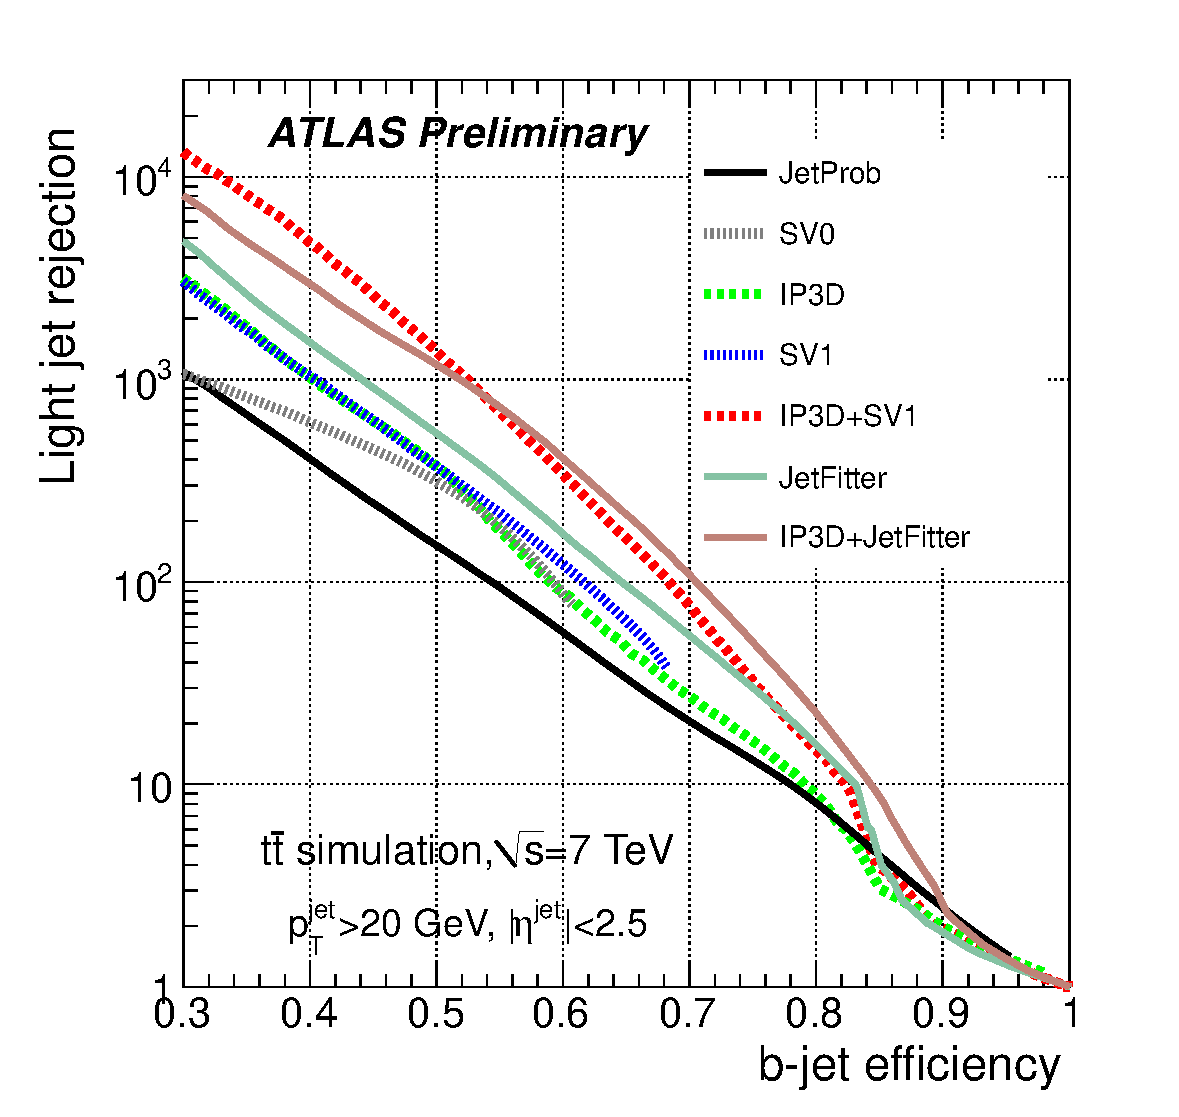
\includegraphics[width=0.75\textwidth]{PartDetector/Plots/DetectorBtaggingPerformanceComp.eps}
  \caption{Light jet rejection as a function of the $b$-jet tagging efficiency, comparing some of taggers used at ATLAS as measured in simulated \ttbar\ events~\cite{Detector:TaggingJetFitter}.}
  \label{fig:DetectorTaggingPerf}
\end{figure}

\subsubsection{The SV0 and SV1 algorithms}

The SV0 algorithm~\cite{Detector:BTaggingSV0} reconstructs secondary vertices using the tracks within the cone of the candidate jet. These secondary vertices are located at a decay length $L$ from the primary vertex. A cut is then applied on the decay length significance $L/\sigma_{L}<5.72$, this is an operating point that yields a $b$-tagging efficiency of $\SI{50}{\percent}$ as measured on simulated inclusive \ttbar\ events.

The SV1 algorithm is an extension of the SV0 algorithm. In order to improve the tagging performance, three properties of the secondary vertex are used as inputs to a likelihood ratio, namely the invariant mass of the tracks associated to the vertex, the ratio of the sum of the energies of the tracks in the vertex to the sum of the energies of the tracks in the jet, and the number of two-track vertices. Additionally the $\DeltaR$ between the jet axis and the line joining the primary and secondary vertices is also used. 

\subsubsection{The JetFitter algorithm}

The JetFitter algorithm~\cite{Detector:TaggingJetFitter} uses a Kalman filter to find a line along which the $b$, $c$ and the primary vertices lie, along with their position on the line, giving an approximated flight-path for the $b$-hadron. Discrimination is based on a likelihood using similar variables as in the SV1 algorithm and additional variables such as the flight length significances of the secondary vertices.

\subsubsection{The IP3D algorithm}

The IP3D algorithm makes use of the transverse and longitudinal impact parameter significances in two-dimensional histograms to discriminate between $b$, $c$ and LF jets. A likelihood-ratio method is used: the IP significances are compared to pre-defined smoothed and normalized distributions for $b$- and light-jets hypotheses. This produces a weight distribution for each model and a cut is applied to select jets. The IP3D algorithm is often combined with the JetFitter (IP3D+JetFitter) or SV1 algorithm (IP3D+SV1) to provide additional discriminating power.

\subsubsection{The MV1 algorithm}

The MV1 algorithm uses the output weights of the IP3D, SV1 and JetFitter algorithms as inputs to an artificial neural network. The current working point used at ATLAS is set at a $b$-tagging efficiency of \SI{70}{\percent} with an associated mistag rate of less than \SI{1.5}{\percent}~\cite{DetectorBtaggingMistagMV1} depending on the $\eta$ and \pt\ of the jet in question.

\subsubsection{Soft Lepton Tagging} \label{sec:DetectorSLT}

\emph{Soft lepton tagging} (SLT) algorithms attempt to identify leptons produced in the semileptonic decay of $b$ and $c$ quarks for the purpose of determining the presence of HF quarks. The term ``semileptonic'' here refers to the decay of a $b$-hadron in such a way as to produce a lepton-neutrino pair along with an additional hadron. The lepton produced would have a low-\pt\ and as such is known as a soft lepton. \mediumtask{Add plot of pt for SMT muon and W muons}\ The SMT tagger exploits muons and as such these will be the focus of the following discussion. 

A soft muon can be produced in a variety of ways starting from a $b$-quark, either directly via $b\rightarrow \mu\bar{\nu}_{\mu}X$, where $X$ is any hadron; or indirectly, via a $c$, $\bar{c}$ or a $\tau$ lepton. The direct and indirect via a $c$ production mechanisms are shown in Figure~\ref{fig:DetectorSLTFeynm}. The branching-ratio for each of these decays is shown in Table~\ref{tab:DetectorSLTBR}. The total BR for the production of a soft muon from a $b$ quark is \SI[multi-part-units=single]{20.1(10)}{\percent}, thus the probability for a \ttbar\ event to contain at least one semileptonic $b$ decay is approximately \SI{36}{\percent}.

\begin{figure}[htbp]
  \centering
    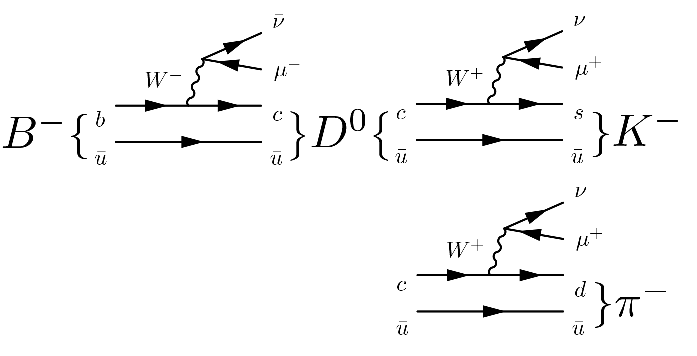
\includegraphics[width=0.75\textwidth]{PartDetector/Diagrams/SemiLeptonicDecay.pdf}
    \caption{Feynman diagram of one of the mechanisms for lepton production via semileptonic $b$ decay. Shown are the direct $b\rightarrow \mu$ and indirect $b\rightarrow c\rightarrow\mu$.}
  \label{fig:DetectorSLTFeynm}
\end{figure}

\begin{table}
  \centering
    \begin{tabular}{@{}lS[table-format=2.2(2)]@{}}
      \toprule
      Mode                                        & {Muon BR [\si{\percent}]} \\
      \midrule % -------------------------
      $b\rightarrow \mu^{-}$                      & {$\num{10.95}\;^{+\;0.29}_{-\;0.25}$} \\
      $b\rightarrow c \rightarrow \mu^{+}$        & 8.02(19) \\
      $b\rightarrow \bar{c} \rightarrow \mu^{-}$  & 1.6(5) \\
      $b\rightarrow \tau^{-} \rightarrow \mu^{-}$ & 0.42(4) \\
      \midrule % -------------------------
      All modes                                   & 21.0(10) \\
      \bottomrule % -------------------------
    \end{tabular}
    \caption{Branching ratio for the production of a muon from a $b$-quark in both direct and indirect modes~\cite{Theory:PDGBooklet}.}
  \label{tab:DetectorSLTBR}
\end{table}

The SLT tagger used in this analysis is based on the quality of the fit between the ID track and MS track as represented by the \xsm. Several tagger-specific cuts are placed on the candidate muons and jet. Candidate SMT muons are required to lie within the coverage of the ID ($|\eta|<2.5$) and have sufficient transverse momentum for reliable reconstruction ($\pt>\SI{4}{GeV}$). Requirements are made on the impact parameters of the muon ID track ($|d_0|<\SI{3}{\mm}$ and $|z_0\sin{\theta}|<\SI{3}{\mm}$) to remove contributions from spurious matches between ID and MS tracks, and from pile-up vertices. Finally, the main cut on the quality of the fit $\xsd=\xsm/\ndof$ is set at less than \num{3.2}. This is an operating point that provides a $b$-jet (semileptonic $b$-jet) identification efficiency of \SI{10}{\percent} (\SI{50}{\percent}) and a LF rejection factor of 200 per jet.

Candidate jets are required to have more than three charged tracks associated with them or a jet EM fraction smaller than \num{0.8}. These criteria ensure that the jet did not originate from the muon itself. Finally, the muon is associated to the jet with a cut $\DeltaR_{\mu}^{\textrm{jet}}<0.5$. The following chapter describes the calibration of the SMT tagger.